Finite element analysis (FEA) is effective at computing stress intensity factors (SIFs) for cracks in complex geometries. However, despite its accuracy, FEA has notable limitations. One significant drawback is its demanding computational requirements, as well as the need for a skilled analyst to achieve reliable results. These factors lead to added time and resource investments, especially for fatigue and uncertainty assessment. To address these challenges, engineers in industry rely on handbook solutions. These solutions offer a practical and efficient way to estimate SIFs for idealized and parameterized crack scenarios and, when applied correctly, they can yield accurate results.


The Raju Newman equations are a widely used set of handbook SIF solutions for various crack shapes and loading conditions \cite{RNeqnsbook}. These handbook are easy to implement in existing workflows as they are closed-form solutions. However, their ease of use sometimes leads to their application in situations that do not align well with the assumptions and limitations of the original idealized model, resulting in inaccurate predictions. This research focuses on the Raju-Newman solution for a semi-elliptical surface crack in a finite plate subjected to mode-I tension. Since its introduction alternative models have been proposed that allow for more complex loading conditions such as the models created by \cite{Wang1995, Pommier1999}. The model crated by Wang and Lambert Follows the same approach used in the Raju-Newman equations of breaking the model into multiple sub-functions. They modified these sub-functions to allow a linear stress function \cite{Wang1995}. Pommier, et al. dropped the useage of Raju-Newman like subfunctions instead opting for a function that directly calculates the boundary  \cite{Pommier1999}. ***********

Machine learning (ML) can play a pivotal role in automating the creation of SIF solutions for more accurate models and more complex geometries. Notably, ML has been successfully employed to produce accurate SIF solutions, as documented in studies such as in \cite{Zhang2023, Sobotka2022, Keprate2017, Xu2022, Seghier2020}. The advantage of ML over other techniques, like those found in \cite{RNeqnsbook, Pommier1999, Wang1995}, is its ability to be trained automatically, resulting in repeatable accurate models. It is worth noting that many commonly used ML algorithms generate "black-box" models, which lack inherent interpretability. In engineering, inherent interpratability in the form of close-form equations allows engineers to easily implement these models into existing modeling codes. inherent interpretability also adds a level of trust to the models. This is why handbook solutions, such as those in \cite{RNeqnsbook}, continue to be used since they inherently offer interpretability. 

ML models have been developed using black box methods as demonstrated by \cite{Keprate2017, Xu2022, Seghier2020}. These ML models, utilizing methods like Gaussian processes regression and neural networks, offer higher accuracy but produce less interpretable models. Notably, the ML models mentioned could predict SIFs at only a single point along the crack front, whereas the Raju-Newman equations can estimate SIFs across the entire crack length.
*********************

While ML models provide improved predictive capabilities, their lack of interpretability can be a drawback in certain contexts, especially when it comes to explaining and trusting the predicted SIF. The interpretability of the Raju and Newman equations gives engineers a clear understanding of how SIFs are derived, aiding decision-making and instilling confidence in the results. Raju and Newman devised a method of breaking down the SIF solution into multiple sub-functions, where each sub-function modifies an analytically solvable case. In the case of a semi-elliptical surface crack the analytical solution to an embedded ellipse in an infinite volume is used. Raju and Newman's approach is detailed in the background section. The method for breaking down the equation provides a framework that can be applied to other crack cases, enhancing the inherent explainability of an analytical solution. 

This research will utilize an interpretable machine learning code Bingo, developed by researchers at NASA and the University of Utah \cite{Randall2022}. Bingo generates closed-form mathematical expressions to predict SIFs along the entire crack length, offering improved accuracy and simplicity compared to the Raju-Newman equations while preserving interpretability. Thanks to the closed-form nature of Bingo's models, they can be easily integrated into existing Linear Elastic Fracture Mechanics (LEFM) software applications like NASGRO, AFGROW, and SMART|DT \cite{nasgro, afgrow, smartdt}.

final paragraph
***************************

\subsection{Background}
In linear elastic fracture mechanics (LEFM), the exact solution for the SIF along an elliptical crack in an infinite volume is given by the equation:

\begin{equation} \label{eqn:K_embedded_ellipse}
    K_{ee} = \sigma \sqrt{\frac{\pi a}{Q}} \left( \sin^2 \phi + \frac{a^2}{c^2} \cos^2 \phi \right)^{1/4} \text{for } a \le c, 
\end{equation}

where $a$ represents the length of the minor axis of the ellipse, $c$ represents the length of the major axis, $\sigma$ is the far-field stress, $\phi$ is the parametric angle of the ellipse, and $Q$ is the square of the complete elliptic integral of the second kind. This expression is only valid when $a \leq c$. In the context of a semi-elliptical surface crack, the values of $a$ and $c$ differ from the minor and major axes, instead representing the crack depth and half-crack surface length, respectively, as illustrated in Fig. \ref{fig:crack_params} \cite{tada1985}. To accommodate cases where $a/c$ will exceed 1, Raju and Newman employed a modified version of equation \ref{eqn:K_embedded_ellipse}. This modification, detailed in Eq. \ref{eqn:fphi}, allows for the use of all values of $a/c$.

\begin{equation} \label{eqn:fphi}
f_{\phi} = \begin{cases}
      \left[\left(\frac{a}{c}\right)^2 \cos^2\phi + \sin^2\phi\right]^{1/4} & \text{if } \frac{a}{c} \le 1 \\
      \\
      \left[\cos^2\phi + \left(\frac{c}{a}\right)^2\sin^2\phi\right]^{1/4} & \text{if } \frac{a}{c} > 1,
    \end{cases}
\end{equation}
 Using Eq. \ref{eqn:K_embedded_ellipse} with Eq. \ref{eqn:fphi} results in Eq. \ref{eqn:K_embedded_ellipse_fphi}

\begin{equation} \label{eqn:K_embedded_ellipse_fphi}
    K_{ee} = \sigma \frac{\sqrt{\pi a}}{E} f_{\phi}.
\end{equation}

 Using Eq. \ref{eqn:K_embedded_ellipse_fphi} and multiplying by the correction factors $f_w$, $M$, and $g$ leads to Eq. \ref{eqn:RN_K},
 \begin{equation} \label{eqn:RN_K}
     K = \frac{\sqrt{\pi a}}{E} f_{\phi} f_w M g,
 \end{equation} 

which models SIFs along the front of a semi-elliptical surface crack in a finite plate.

The finite width correction factor $f_w$,
\begin{equation} \label{eqn:RN_fw}
    f_w = \sqrt{\sec\left(\frac{\pi c}{2b}\sqrt{\frac{a}{t}}\right)},
\end{equation}
 is a 3D extension for the equation developed in \cite{brown1966}, which accounts for the finite width and thickness of the plate when $a/c = 1$ and $\phi = \pi/2$. The thickness of the plate is denoted as $t$ and the half-width of the plate is denoted as $b$ Fig. \ref{fig:crack_params}. The function $M$ accounts for changes in SIF due to the aspect ratio of the crack at the point along the crack where $\phi = \pi/2$ and is given by
 
 \begin{figure}%
 	\centering
 	\subfloat[\centering Crack dimensions]{{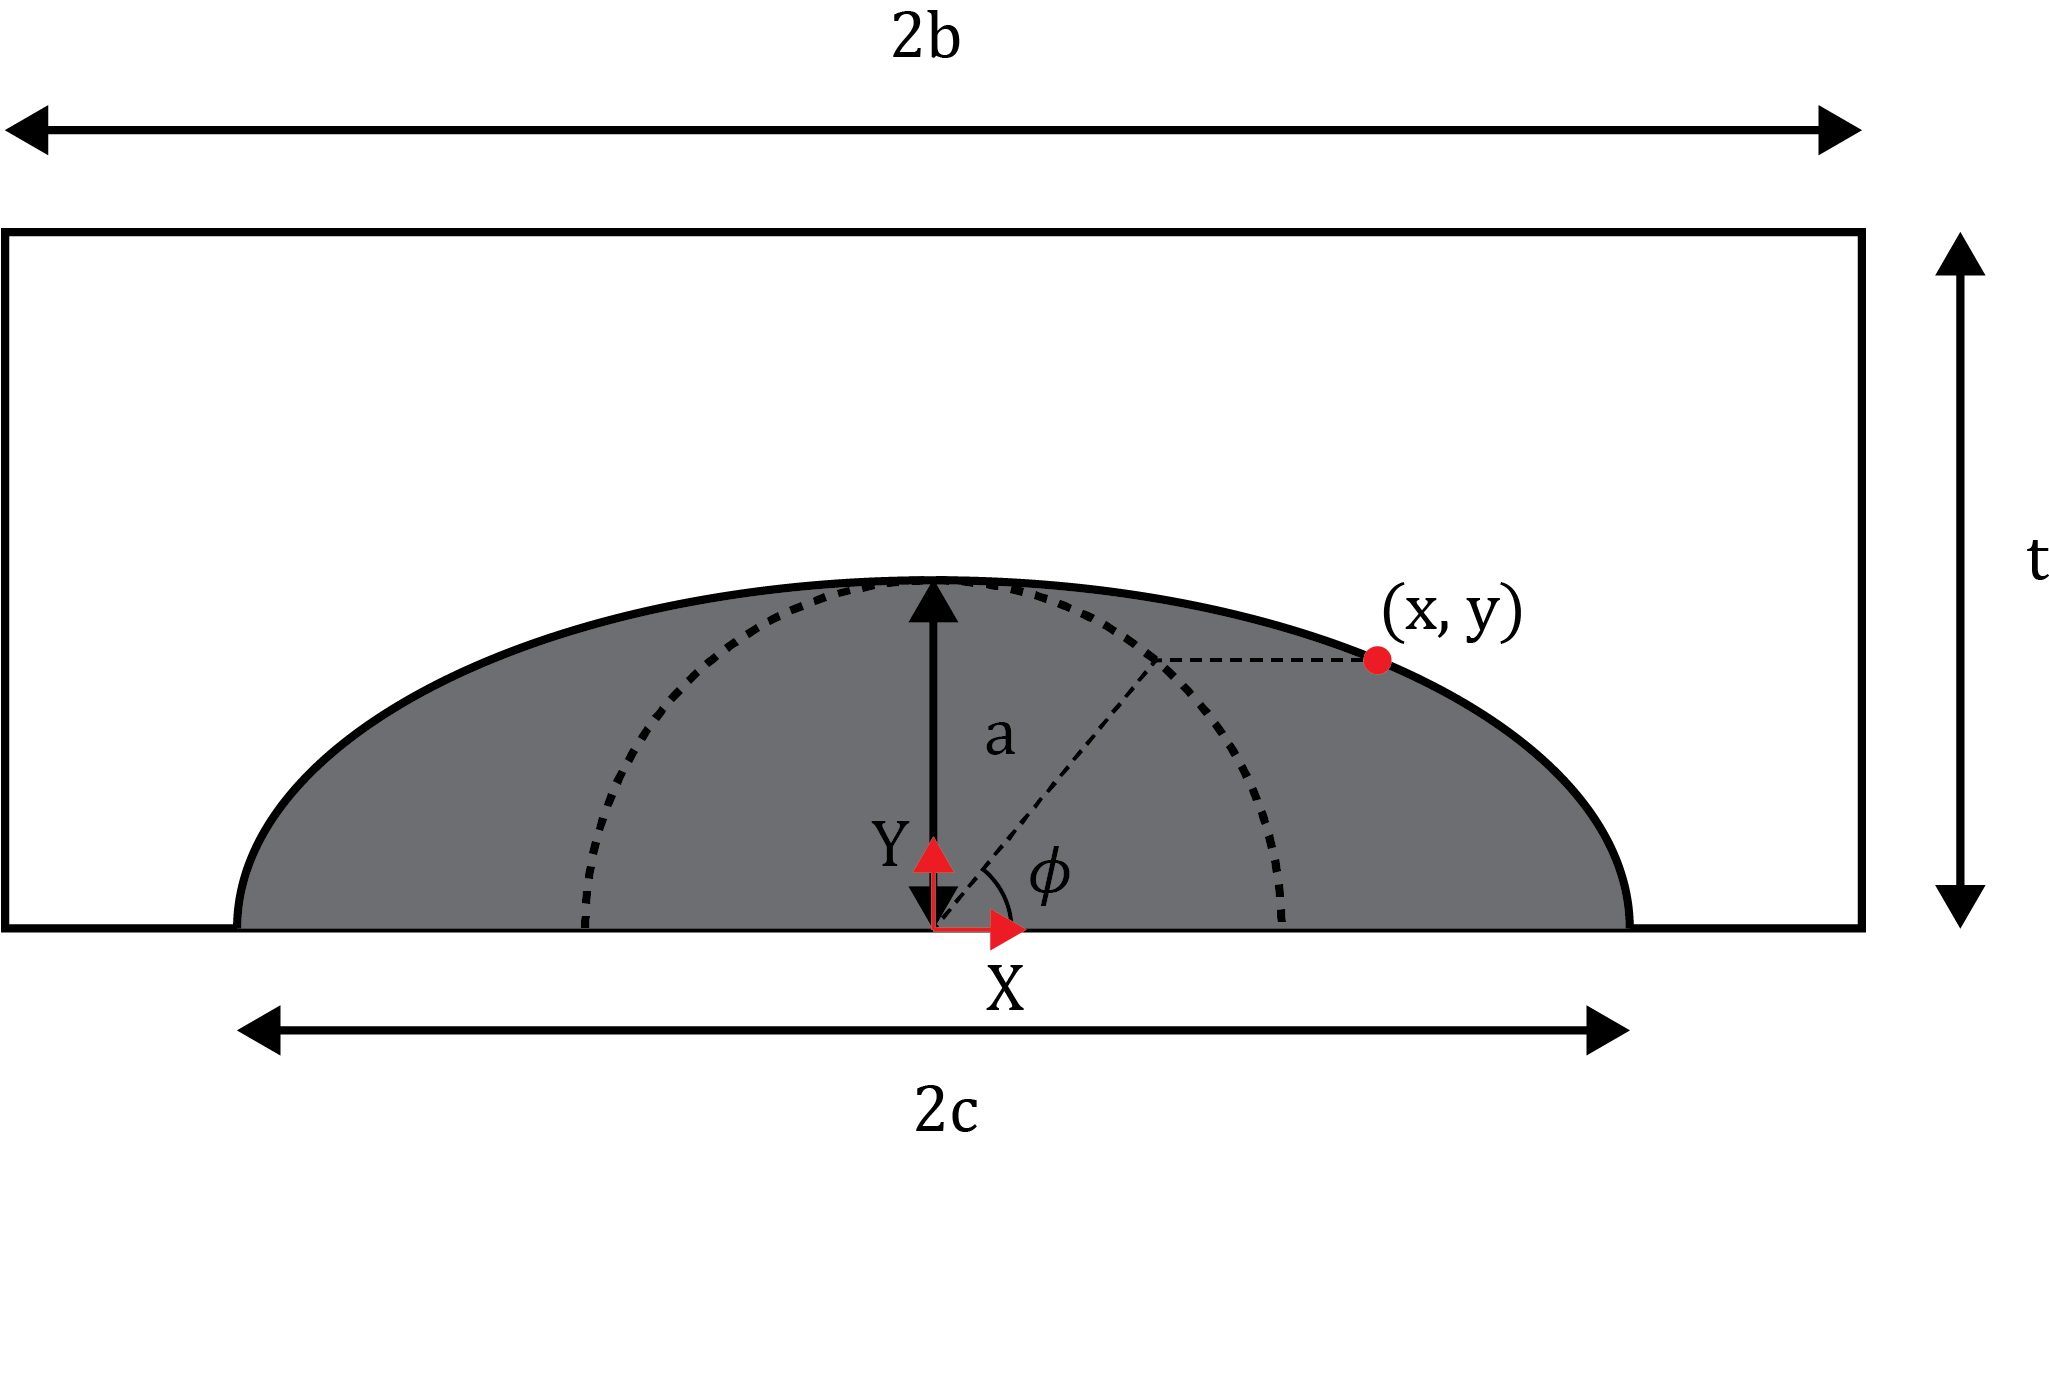
\includegraphics[width=0.5\textwidth]{geometry_figures/params.png} }}%
 	\qquad
 	\subfloat[\centering Ellipse dimensions]{{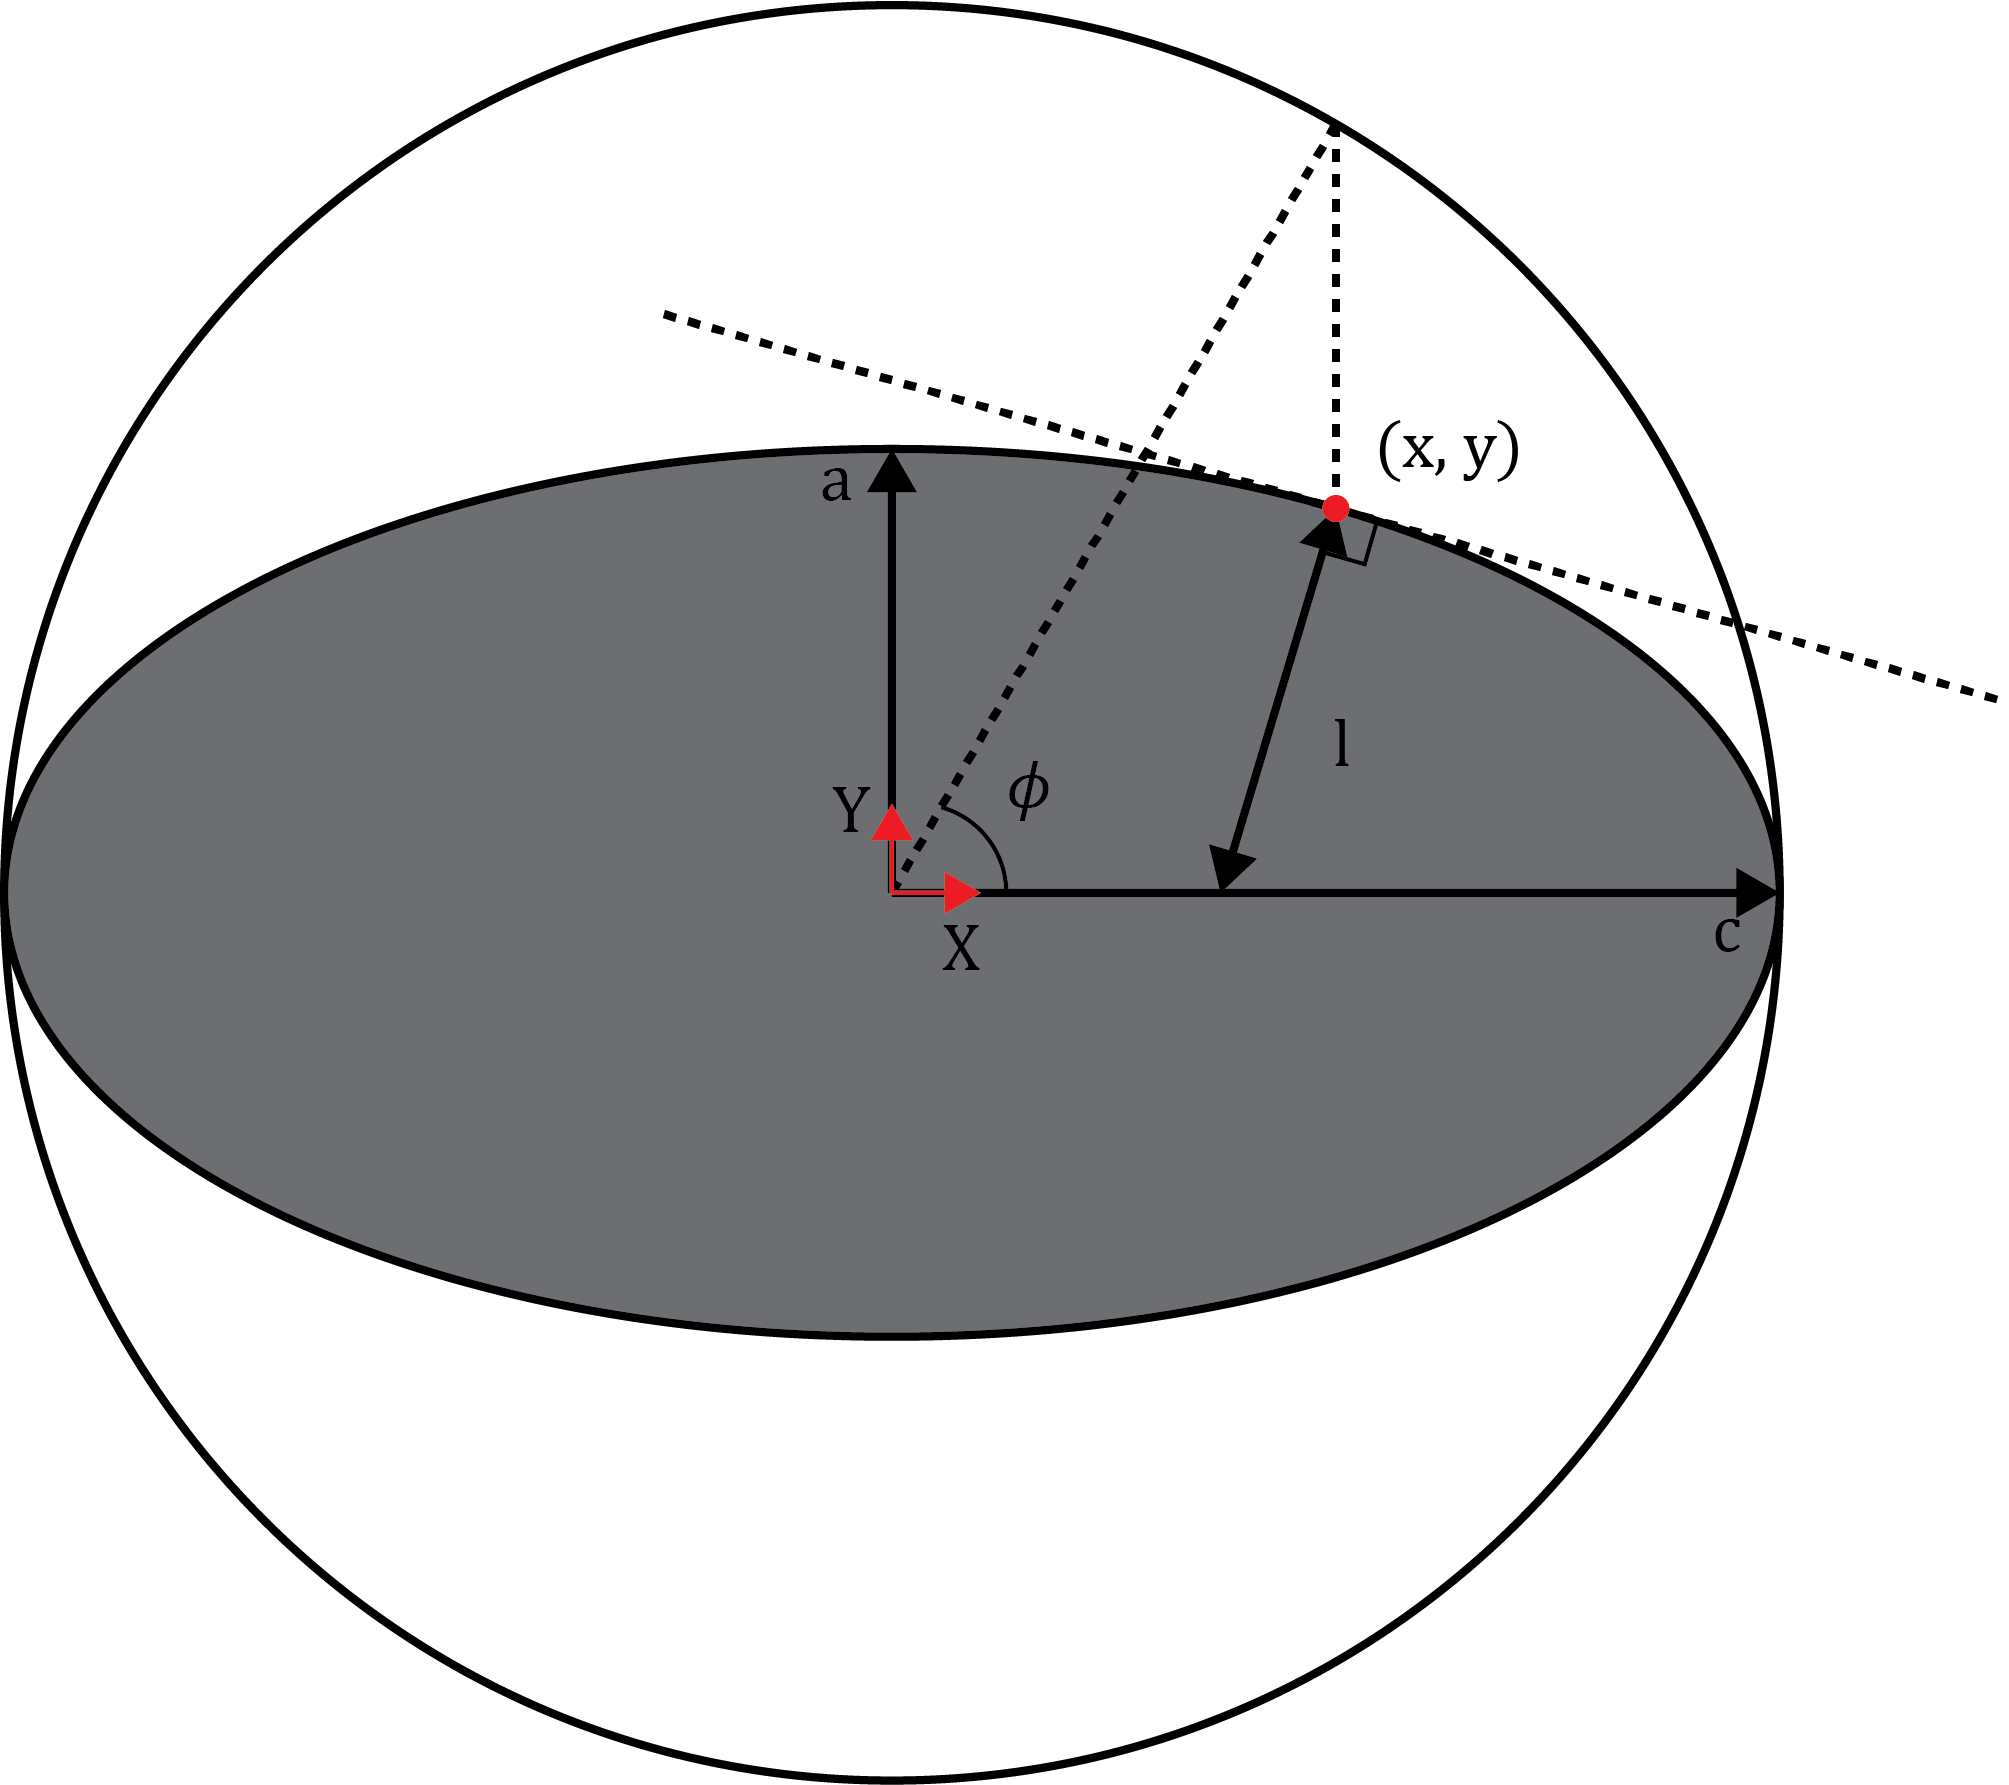
\includegraphics[width=0.5\textwidth]{geometry_figures/Ellipse.png} }}%
 	\caption{(a) Crack parameters with $a$ being the crack depth and $2c$ being the surface crack length. (b) $\phi$ is defined by the angle to the inscribed circle projected to the ellipse. $l$ is defined as the distance perpendicular to the tangent line from the point of interest to the nearest axis.}%
 	\label{fig:crack_params}%
 \end{figure}
\begin{equation} \label{eqn:RN_M}
    M = M_1 + M_2\left(\frac{a}{t}\right)^2 + M_3\left(\frac{a}{t}\right)^4, \text{ where}
\end{equation}
\begin{equation} \label{eqn:RN_M1}
    M_1 = \begin{cases}
    1.13 - 0.09\left(\frac{a}{c}\right) & \text{if } \frac{a}{c} \le 1 \\
    \\
    \sqrt{\frac{c}{a}}\left(1 + 0.04\frac{c}{a}\right) & \text{if } \frac{a}{c} > 1
    \end{cases}
\end{equation}
\begin{equation} \label{eqn:RN_M2}
    M_2 = \begin{cases}
    -0.54 + \frac{0.89}{0.2+\left(\frac{a}{c}\right)} & \text{if } \frac{a}{c} \le 1 \\
    \\
    0.2\left(\frac{c}{a}\right)^4 & \text{if } \frac{a}{c} > 1
    \end{cases}
\end{equation}
\begin{equation} \label{eqn:RN_M3}
    M_3 = \begin{cases}
    0.5 - \frac{1}{0.65+\frac{a}{c}} + 14\left(1-\frac{a}{c}\right)^{24} & \text{if } \frac{a}{c} \le 1 \\
    \\
    -0.11\left(\frac{c}{a}\right)^4 & \text{if } \frac{a}{c} > 1.
    \end{cases}
\end{equation}
The function g corrects for free surface effects and is denoted by
\begin{equation} \label{eqn:RN_g}
    g = \begin{cases}
    1 + \left[0.1 + 0.35\left(\frac{a}{t}\right)^2\right]\left(1 - \sin\phi\right)^2 & \text{if } \frac{a}{c} \le 1 \\
    \\
    1 + \left[0.1 + 0.35\left(\frac{c}{a}\right)\left(\frac{a}{t}\right)^2\right]\left(1 - \sin\phi\right) & \text{if } \frac{a}{c} > 1.
    \end{cases}
\end{equation}
The function $g$ is sinusoidal, having a value of 1 at $\phi = \pi/2$.  By using this methodical approach of breaking down the problem into sub-functions that each account for a different aspect of the crack, allowed Raju and Newman to develop accurate equations that build upon the explainablity from the analytical solution of the embedded ellipse. 
